\chapter{Multidimensional Data Organizations}


Let us consider multidimensional data representing points or regions in a \textit{k}-dimensional space.
For example, the \textit{k} attributes of the records of a relation can be interpreted as coordinates of a \textit{k}-dimensional space and a table of $N_{rec}$ record as $N_{rec}$ spatial points.

Consider a set of 8 records with two attributes $A_1$ as latitude and $A_2$ as longitude of cities, both normalized in the range 0 to 100.

\begin{figure}[!htb]
    \begin{minipage}{0.48\textwidth} 
     \centering
     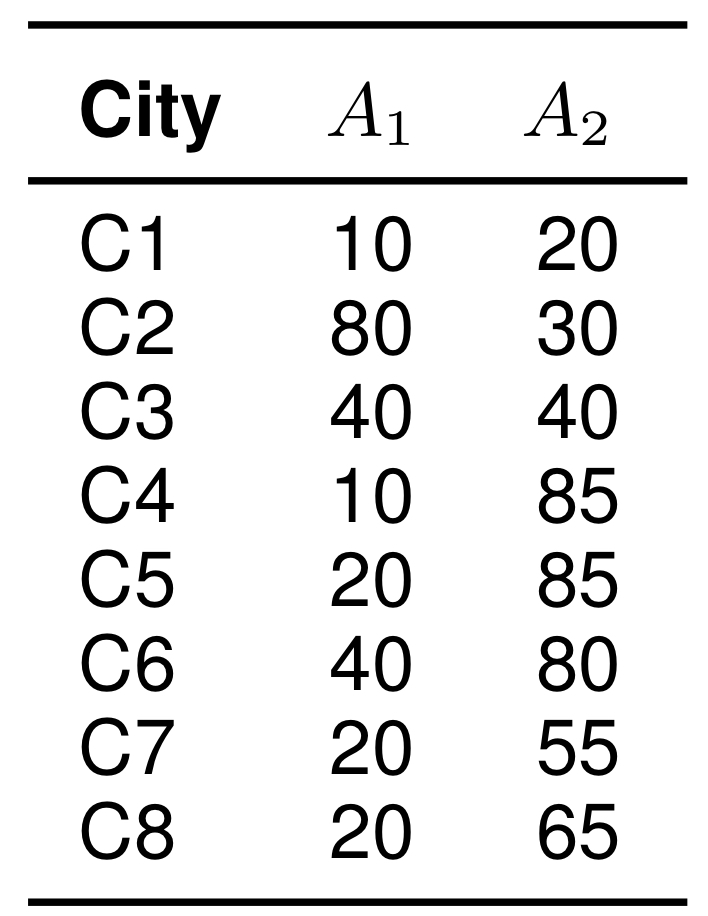
\includegraphics[width=0.5\textwidth]{images/DBMS_Internals/MultiDimensionalDataOrganizations/mutidimdata2.jpeg}
     \caption{Multidimensional representation of data on cities}
   \end{minipage}\hfill
   \begin{minipage}{0.48\textwidth}
     \centering
     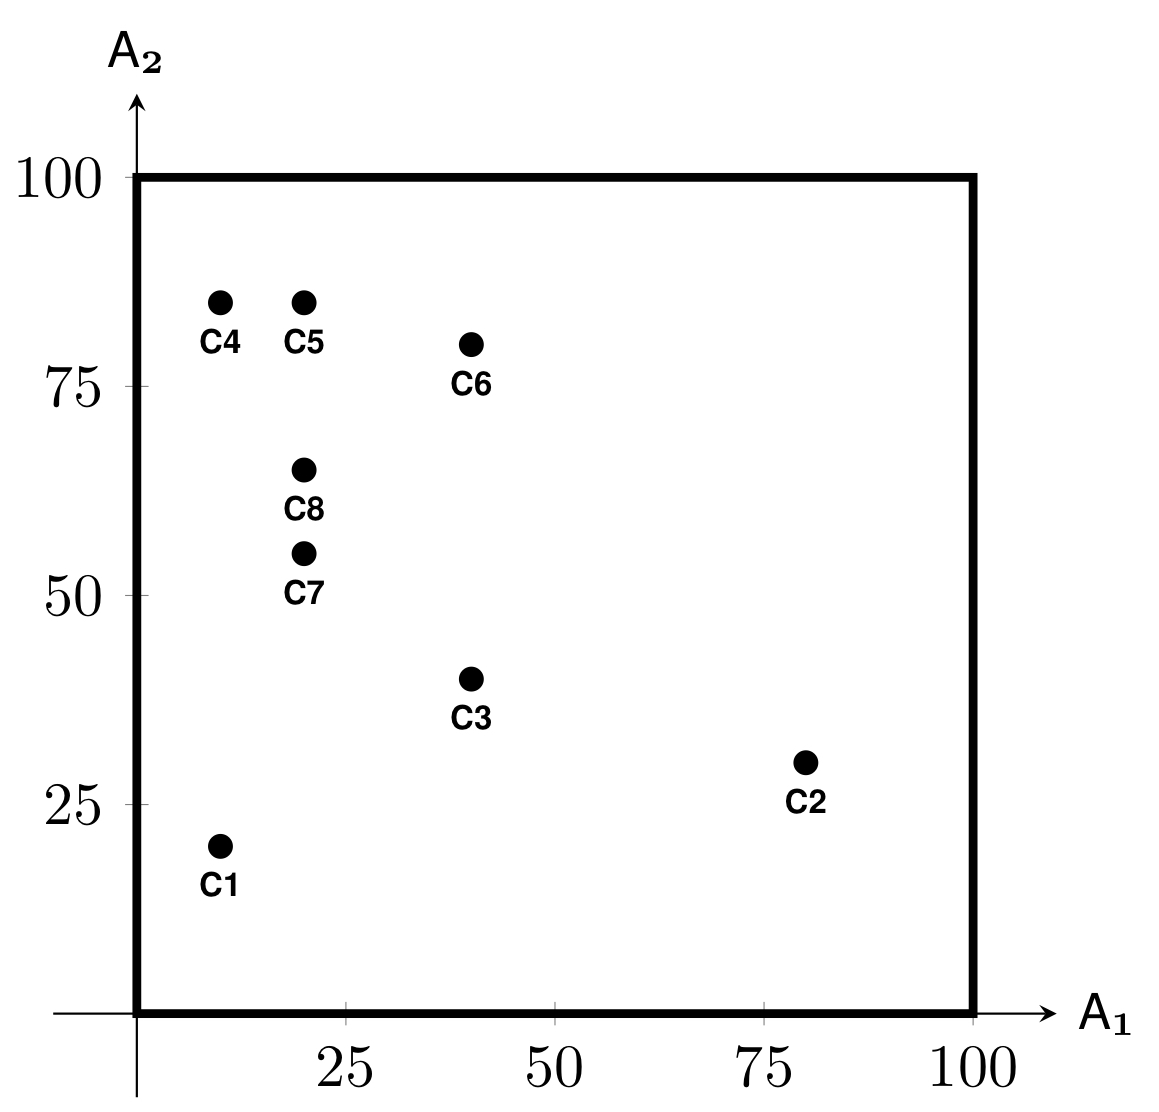
\includegraphics[width=\textwidth]{images/DBMS_Internals/MultiDimensionalDataOrganizations/multidimdata.jpeg}
     \caption{Data on cities locations}
   \end{minipage}
\end{figure}


The problems that will be considered are:
\begin{enumerate}
    \item \textbf{(Primary organization)} How to divide stored data across pages?
    \item \textbf{(Secondary organization)} How to divide index entries across index levels?
\end{enumerate}

The two questions depends on the type of queries supported:
\begin{itemize}
    \item \textit{Point / region search:} check if point/region is present
    \item \textit{Spatial range search:} points/regions in a (hyper)rectangle or (hyper)ball
    \item \textit{k-Nearest neighbors (k-NN):} k points/regions that are the closest ones with respect to a selected point/region
\end{itemize}
 
We have multiple choice in order to split our data in a multidimensional organizations, like:
\begin{itemize}
    \item \textbf{Linear} order based organizations, traditional indexes to map the position
    \begin{itemize}
        \item How to build a total order on multidimensional data?
    \end{itemize}
    \item Space \textbf{partitioning} organizations, referred to the hash approach 
    \begin{itemize}
        \item How to partition the space in regions that contain records that can be stored in a page?
        \item How to quickly find the region containing the points in a specified rectangular area?
    \end{itemize}
    \item \textbf{Generalized search tree} based organizations, forget about the space and it focus on the data, it divide the point s to build something that is easy to search
    \begin{itemize}
        \item How to choose (overlapping) regions that contain record to be stored in a page?
        \item How to quickly find region(s) containing the points for a specific query?
    \end{itemize}
\end{itemize}


\section{Linearization- B$^+$-tree}
\begin{itemize}
    \item \textbf{Multi-attribute lexicographic order}
    \begin{itemize}
        \item The dotted lines indicate the linear order in which points are stored in a B+–tree
        \item The boxes how points are stored in a multidimensional index
        \item Good for point search
        \item Almost useless for range search and k-NN. Because depending on the key we are not even able to find a single interesting page
    \end{itemize}
    \begin{figure}[h]
         \centering
         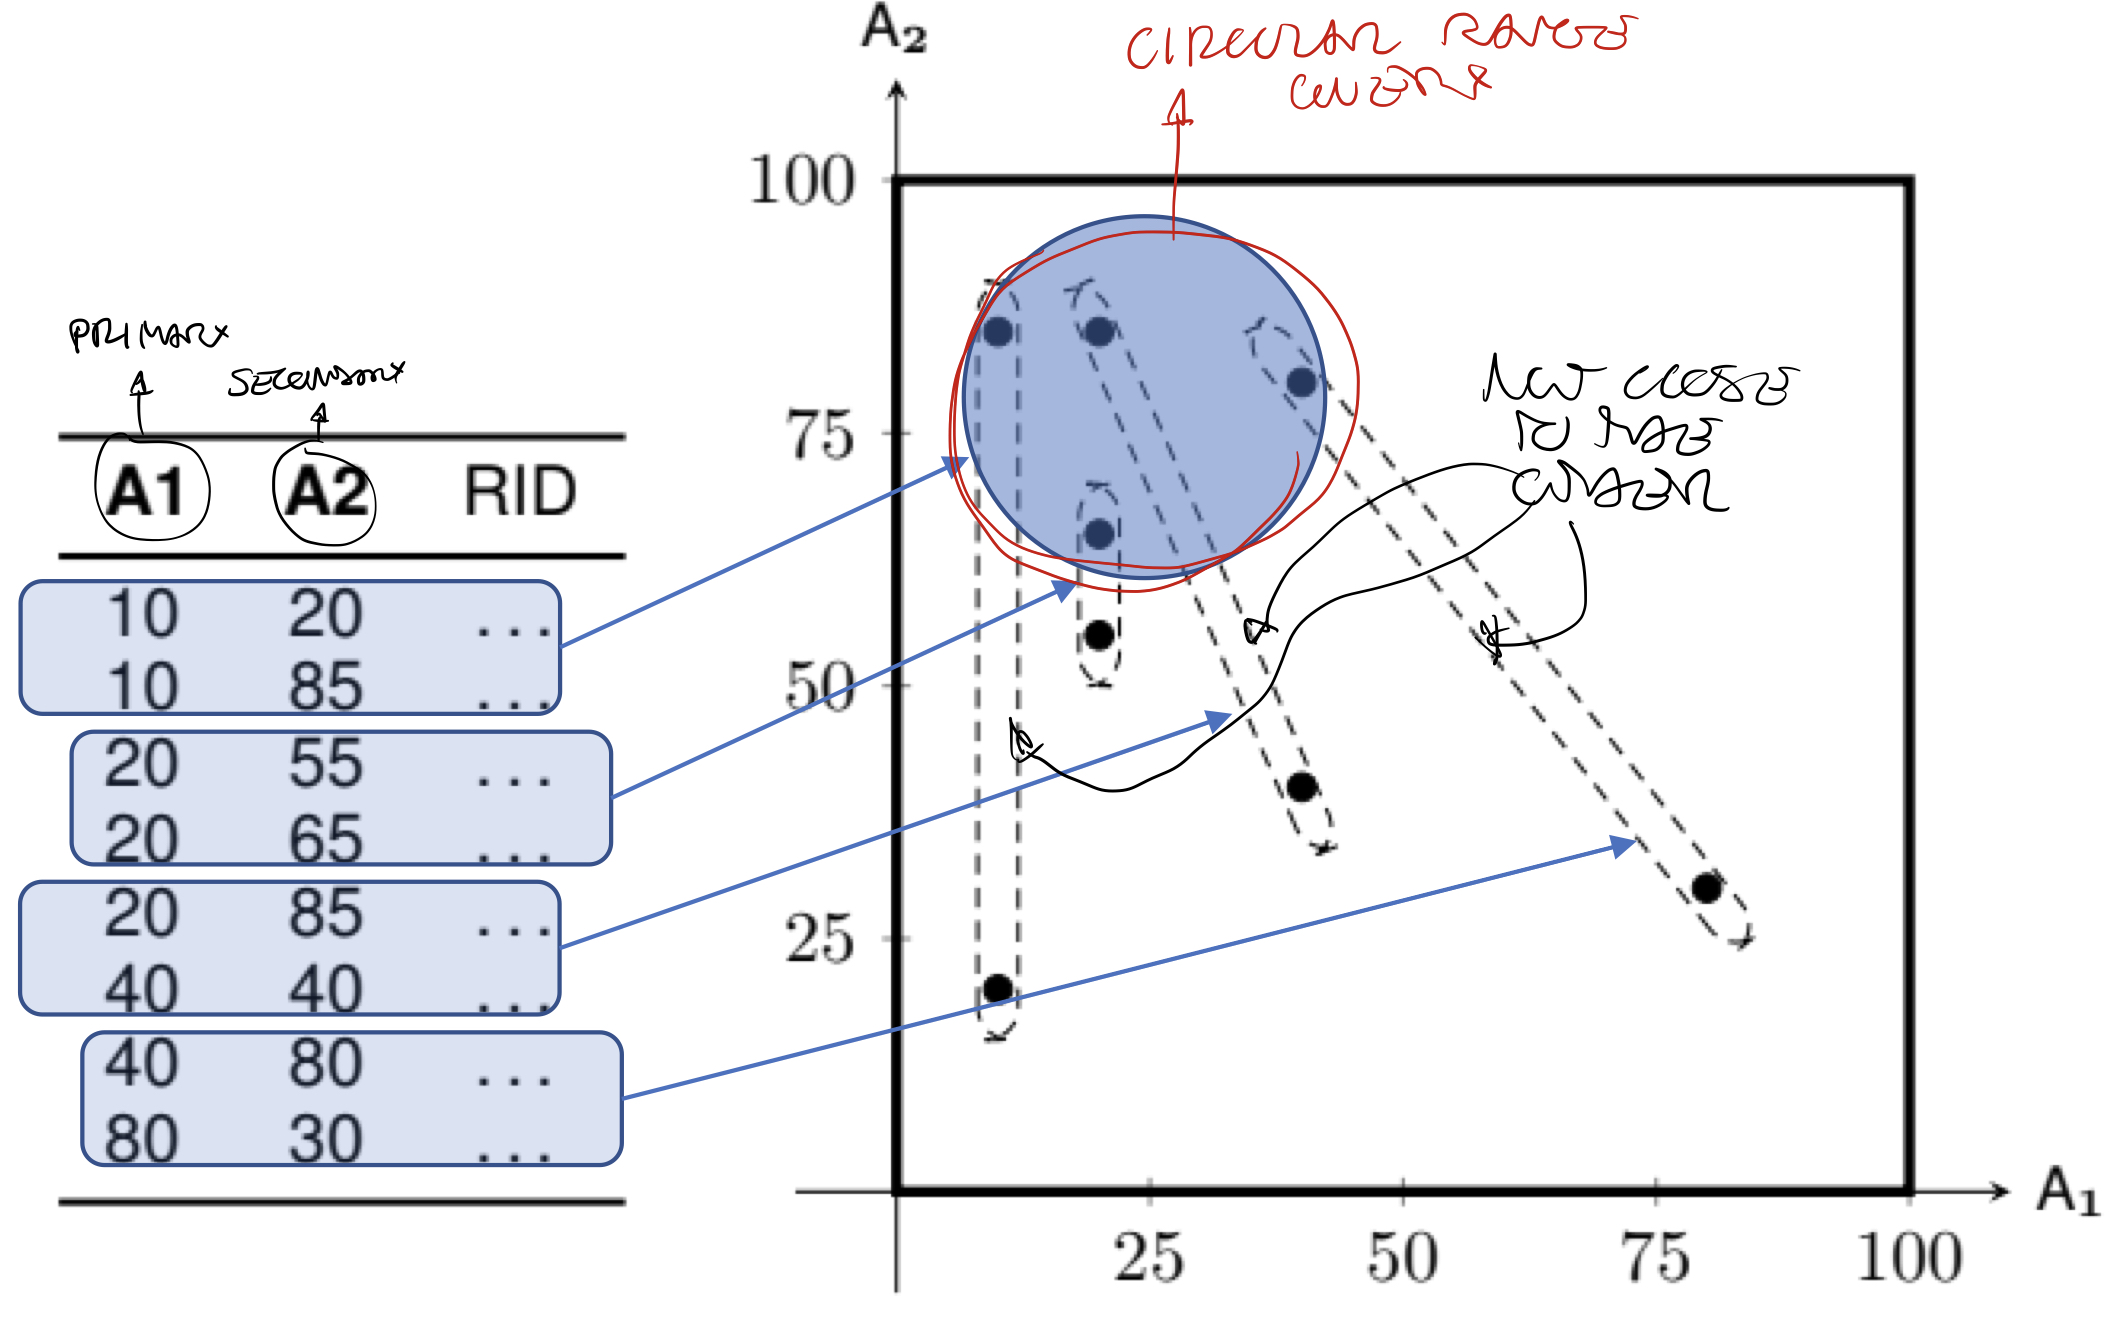
\includegraphics[width=.5\linewidth]{images/DBMS_Internals/MultiDimensionalDataOrganizations/multi-att-lexigo.jpeg}
    \end{figure}
    
    \newpage
    \item \textbf{Diagonal order (sum of coordinates)}
    \begin{figure}[h]
         \centering
         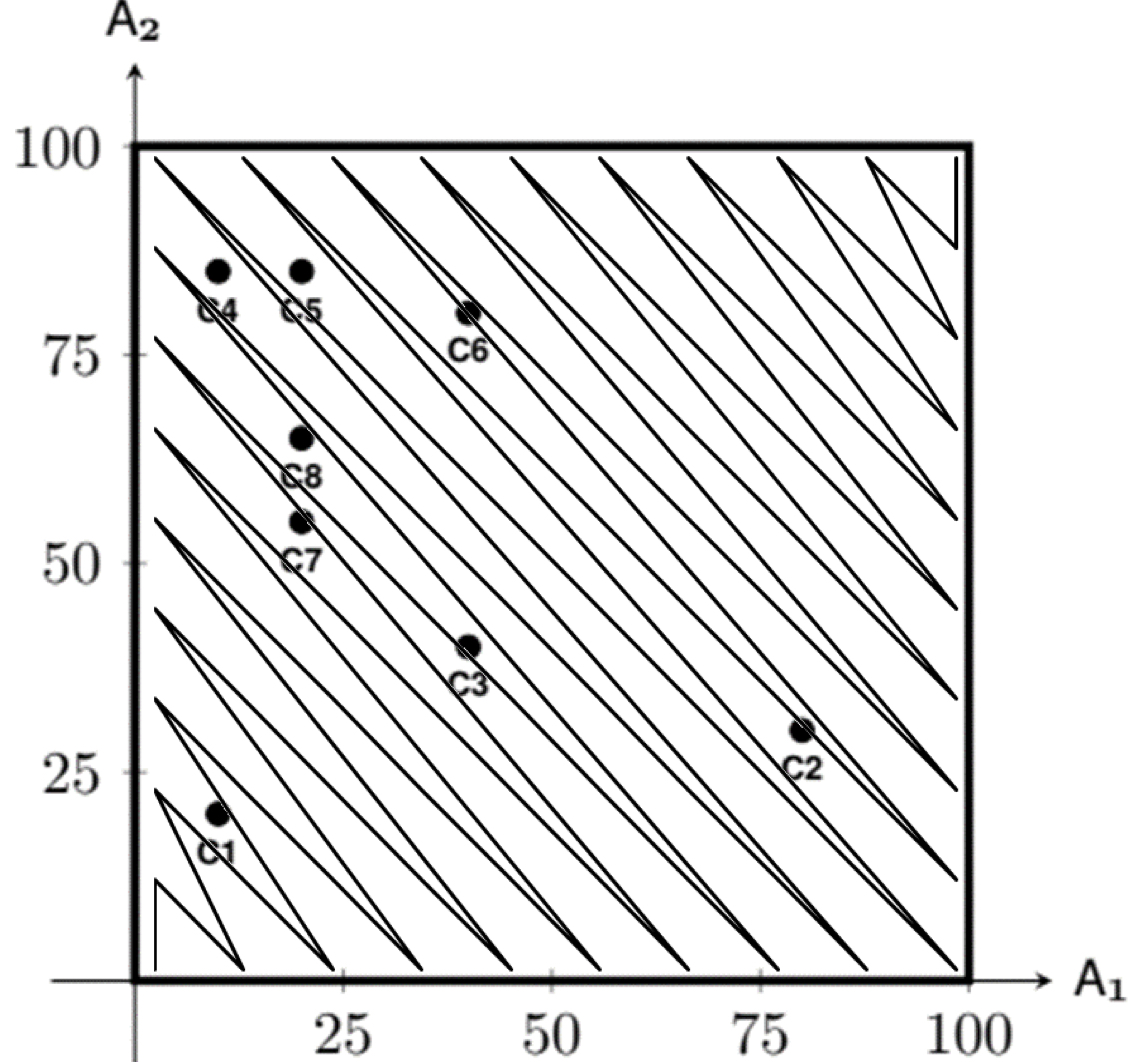
\includegraphics[width=.4\linewidth]{images/DBMS_Internals/MultiDimensionalDataOrganizations/diagonal_order.jpeg}
    \end{figure}

    
    \item \textbf{Morton space filling curve, Z-order}
    \begin{figure}[h]
         \centering
         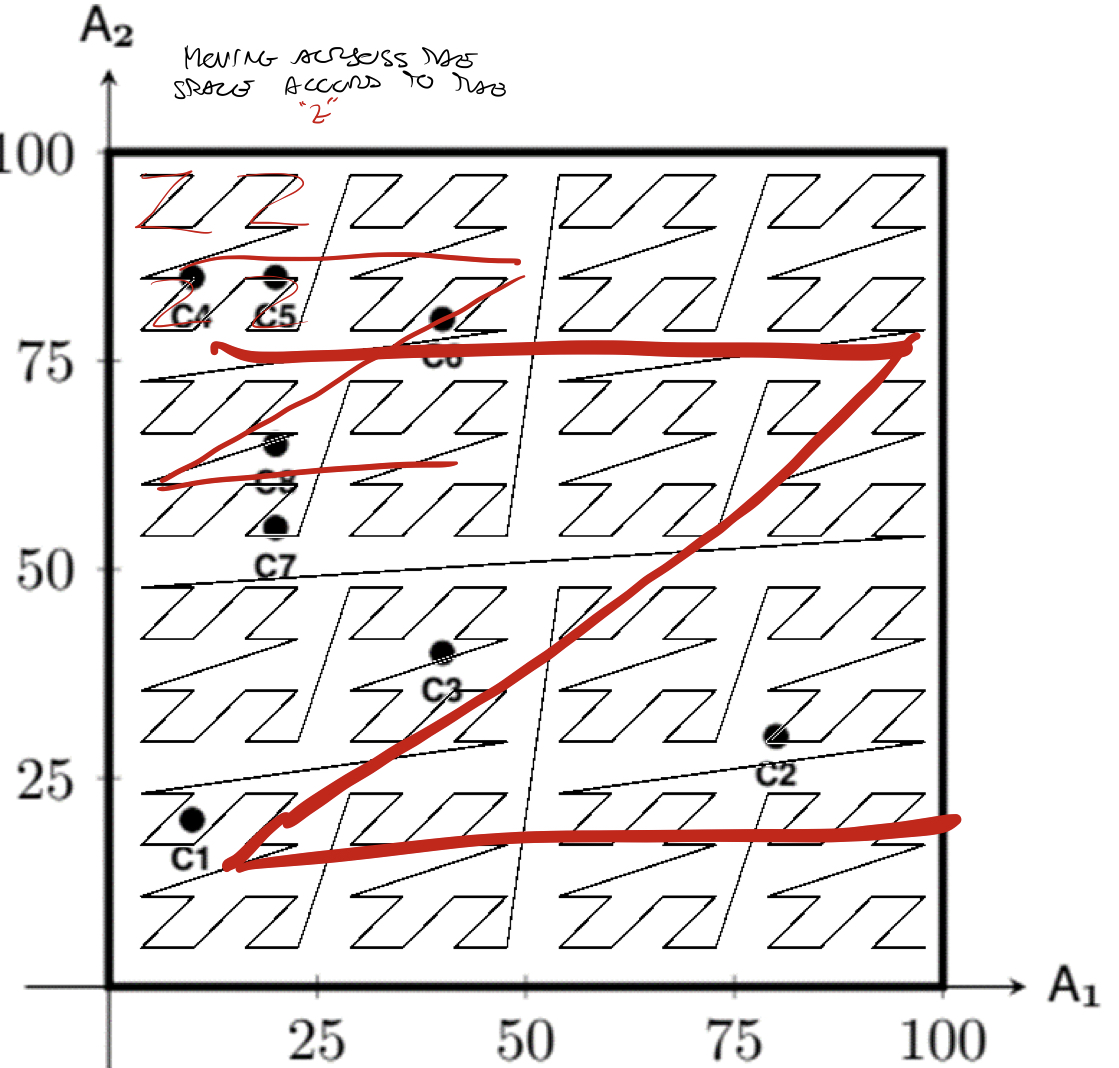
\includegraphics[width=.4\linewidth]{images/DBMS_Internals/MultiDimensionalDataOrganizations/z_order.jpeg}
    \end{figure}

    
    \item \textbf{Peano space filling curve}
    \begin{figure}[h]
         \centering
         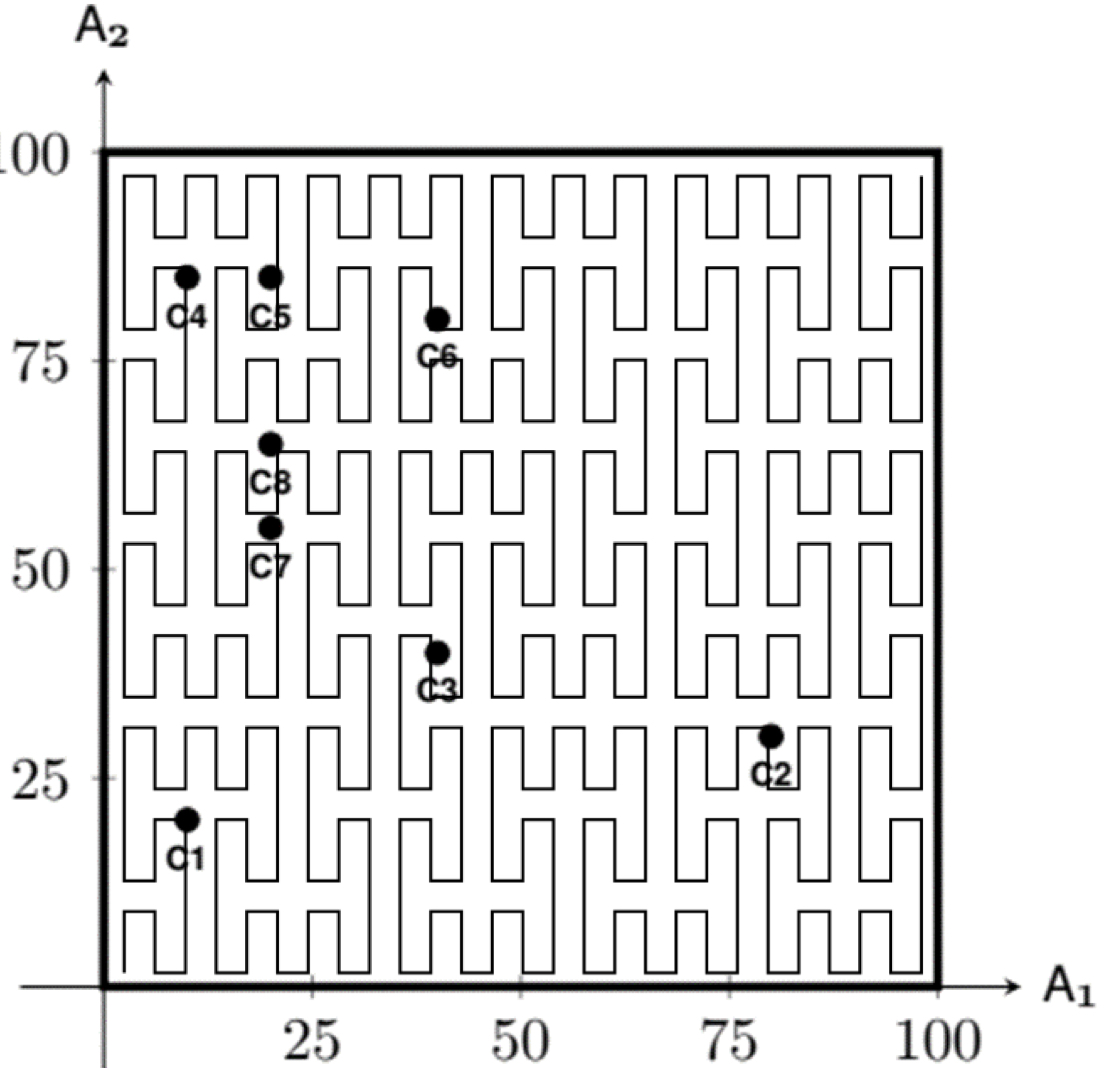
\includegraphics[width=.4\linewidth]{images/DBMS_Internals/MultiDimensionalDataOrganizations/peano.jpeg}
    \end{figure}

    
    \item \textbf{Hilbert space filling curve}
    \begin{figure}[h]
         \centering
         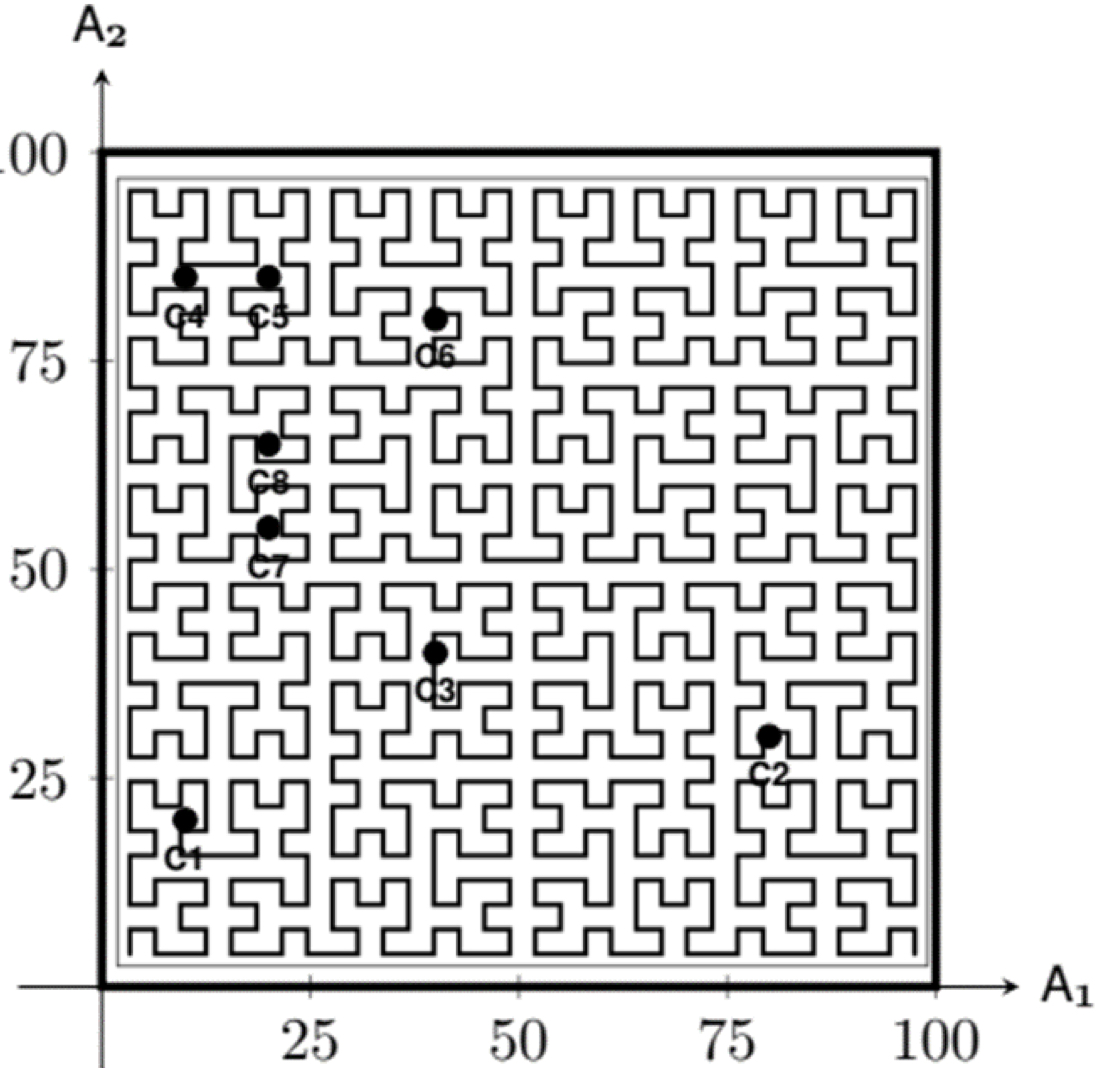
\includegraphics[width=.4\linewidth]{images/DBMS_Internals/MultiDimensionalDataOrganizations/hilbert.jpeg}
    \end{figure}

    
\end{itemize}

\subsection{Space partitioning}
\begin{itemize}
    \item \textbf{Classical}
    \begin{itemize}
        \item Suppose that pages have a capacity 2 and we want to load the data on cities. After the insertion of “C1” and “C2”, the insertion of “C3” requires distributing the data into two pages. 
        \item To proceed let us divide the data space into non-overlapping partitions according to the first coordinate by choosing a value of separation $d$ for $A_1$: points with coordinate $A_1 \leq d$ are inserted into a page, those with a higher value are inserted into another one.
        \item When there is a new overflow from a page during data loading, we proceed with another split of the partition, but changing the reference coordinate, with the logic that the splitting dimension alternates.
        
        \begin{figure}[h]
         \centering
         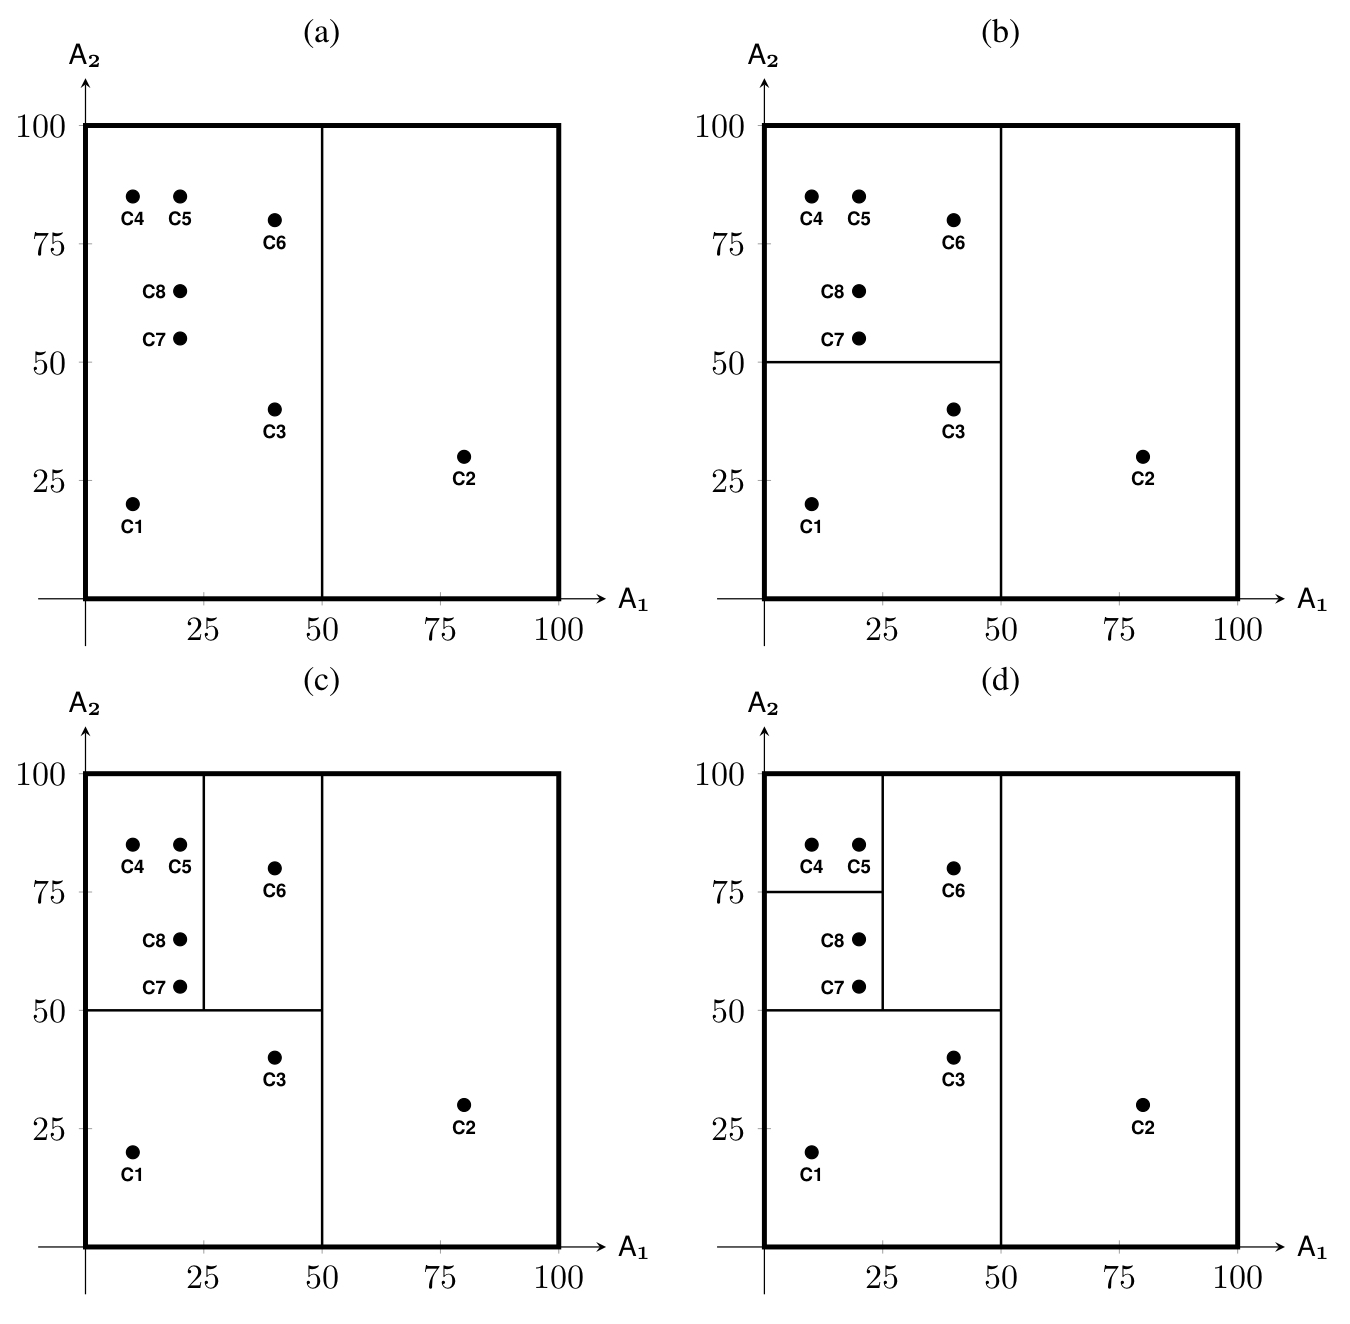
\includegraphics[width=.5\linewidth]{images/DBMS_Internals/MultiDimensionalDataOrganizations/partitioning.jpeg}
        \end{figure}
        
        \end{itemize}

    \newpage
    \item \textbf{Point region quadtrees}
    \begin{itemize}
        \item Used to organize bidimensional data, evolution of the binary tree to 2D
        \item 2 thresholds splits the domain in 4 parts, reason of the name
        
        \begin{figure}[h]
         \centering
         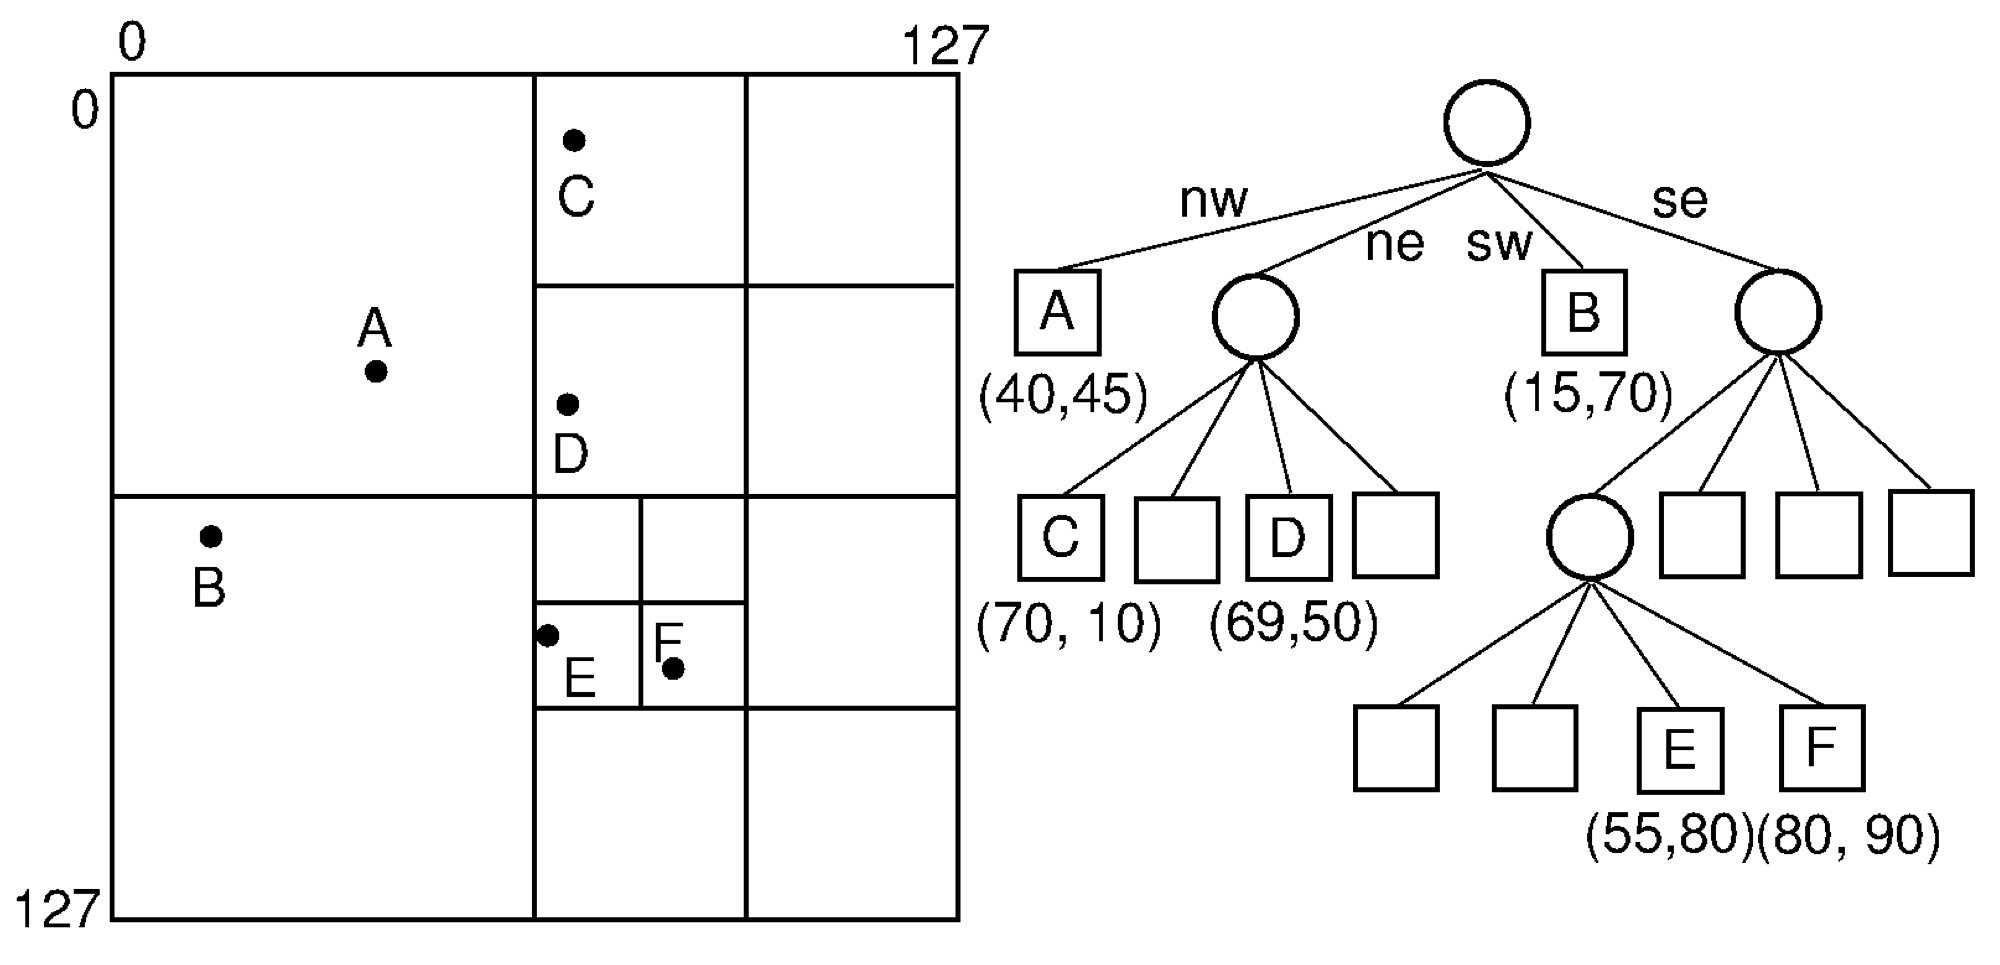
\includegraphics[width=.5\linewidth]{images/DBMS_Internals/MultiDimensionalDataOrganizations/quadtrees.jpeg}
        \end{figure}
        
    \end{itemize}
    
    \item \textbf{Octrees}
    \begin{itemize}
        \item Create regions that are not new
        \item Higher is the dimension, higher will be the number of nodes that we have to generate 
        \item Splitting in the middle could be not the best choice 
        
        \begin{figure}[h]
         \centering
         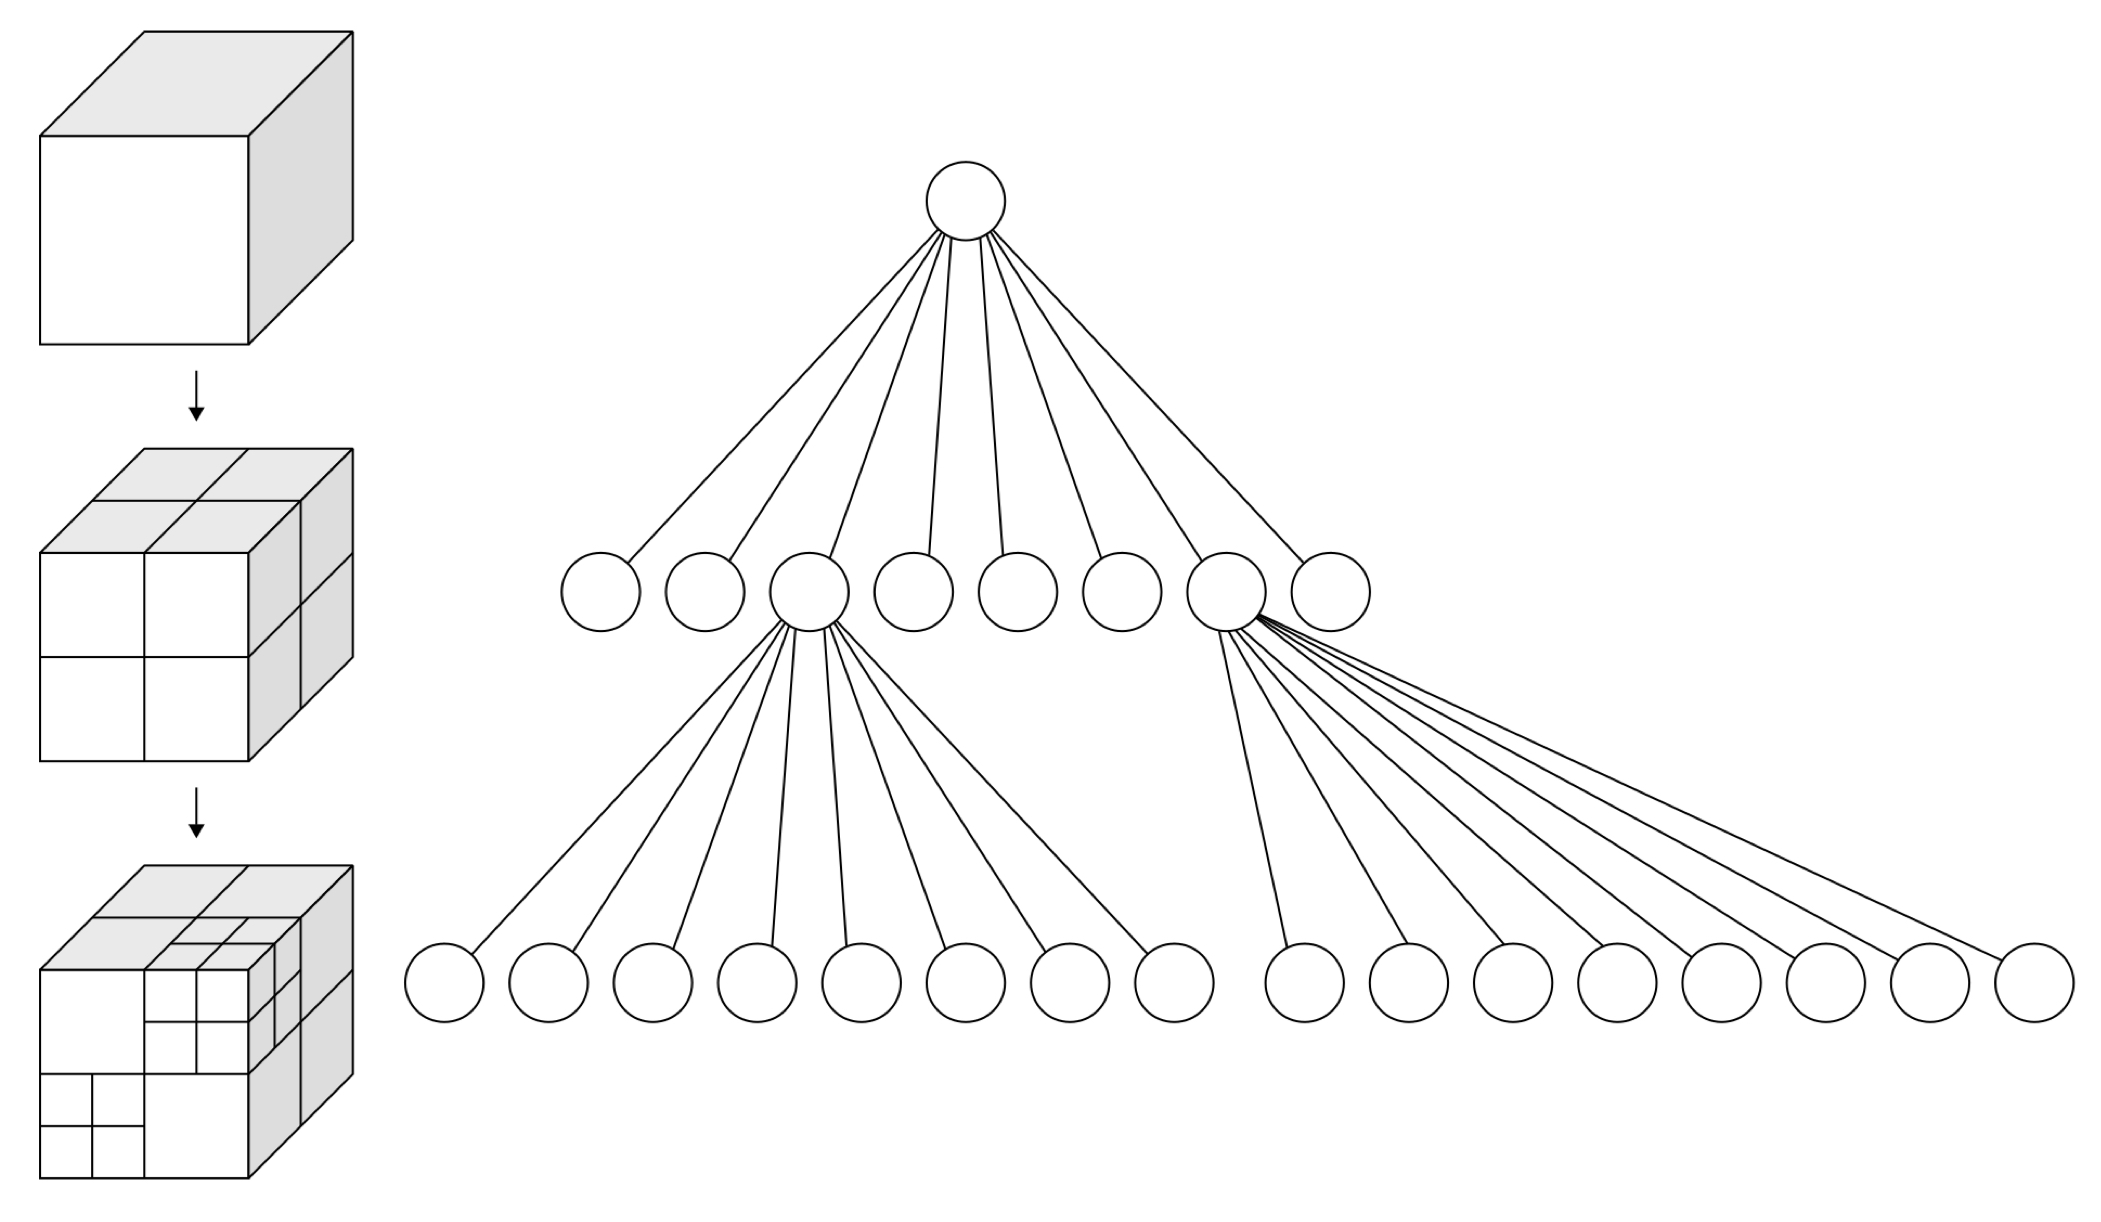
\includegraphics[width=.5\linewidth]{images/DBMS_Internals/MultiDimensionalDataOrganizations/octrees.jpeg}
    \end{figure}
        
    \end{itemize}

    \newpage
    \item \textbf{KDB-trees}
    \begin{itemize}
        \item Inherit the idea to have a threshold to split the domain, but it uses a coordinate at time and we circle the order of splitting strategy
        \item Every part is splitted when needed
        \item How do we find which is the right position? 
        \begin{itemize}
            \item Start from the root is easy
            \item Start from bottom $\rightarrow$ additional tree to take care on the partition volume: \textbf{G-trees}
        \end{itemize}
    \end{itemize}

    \begin{figure}[h]
         \centering
         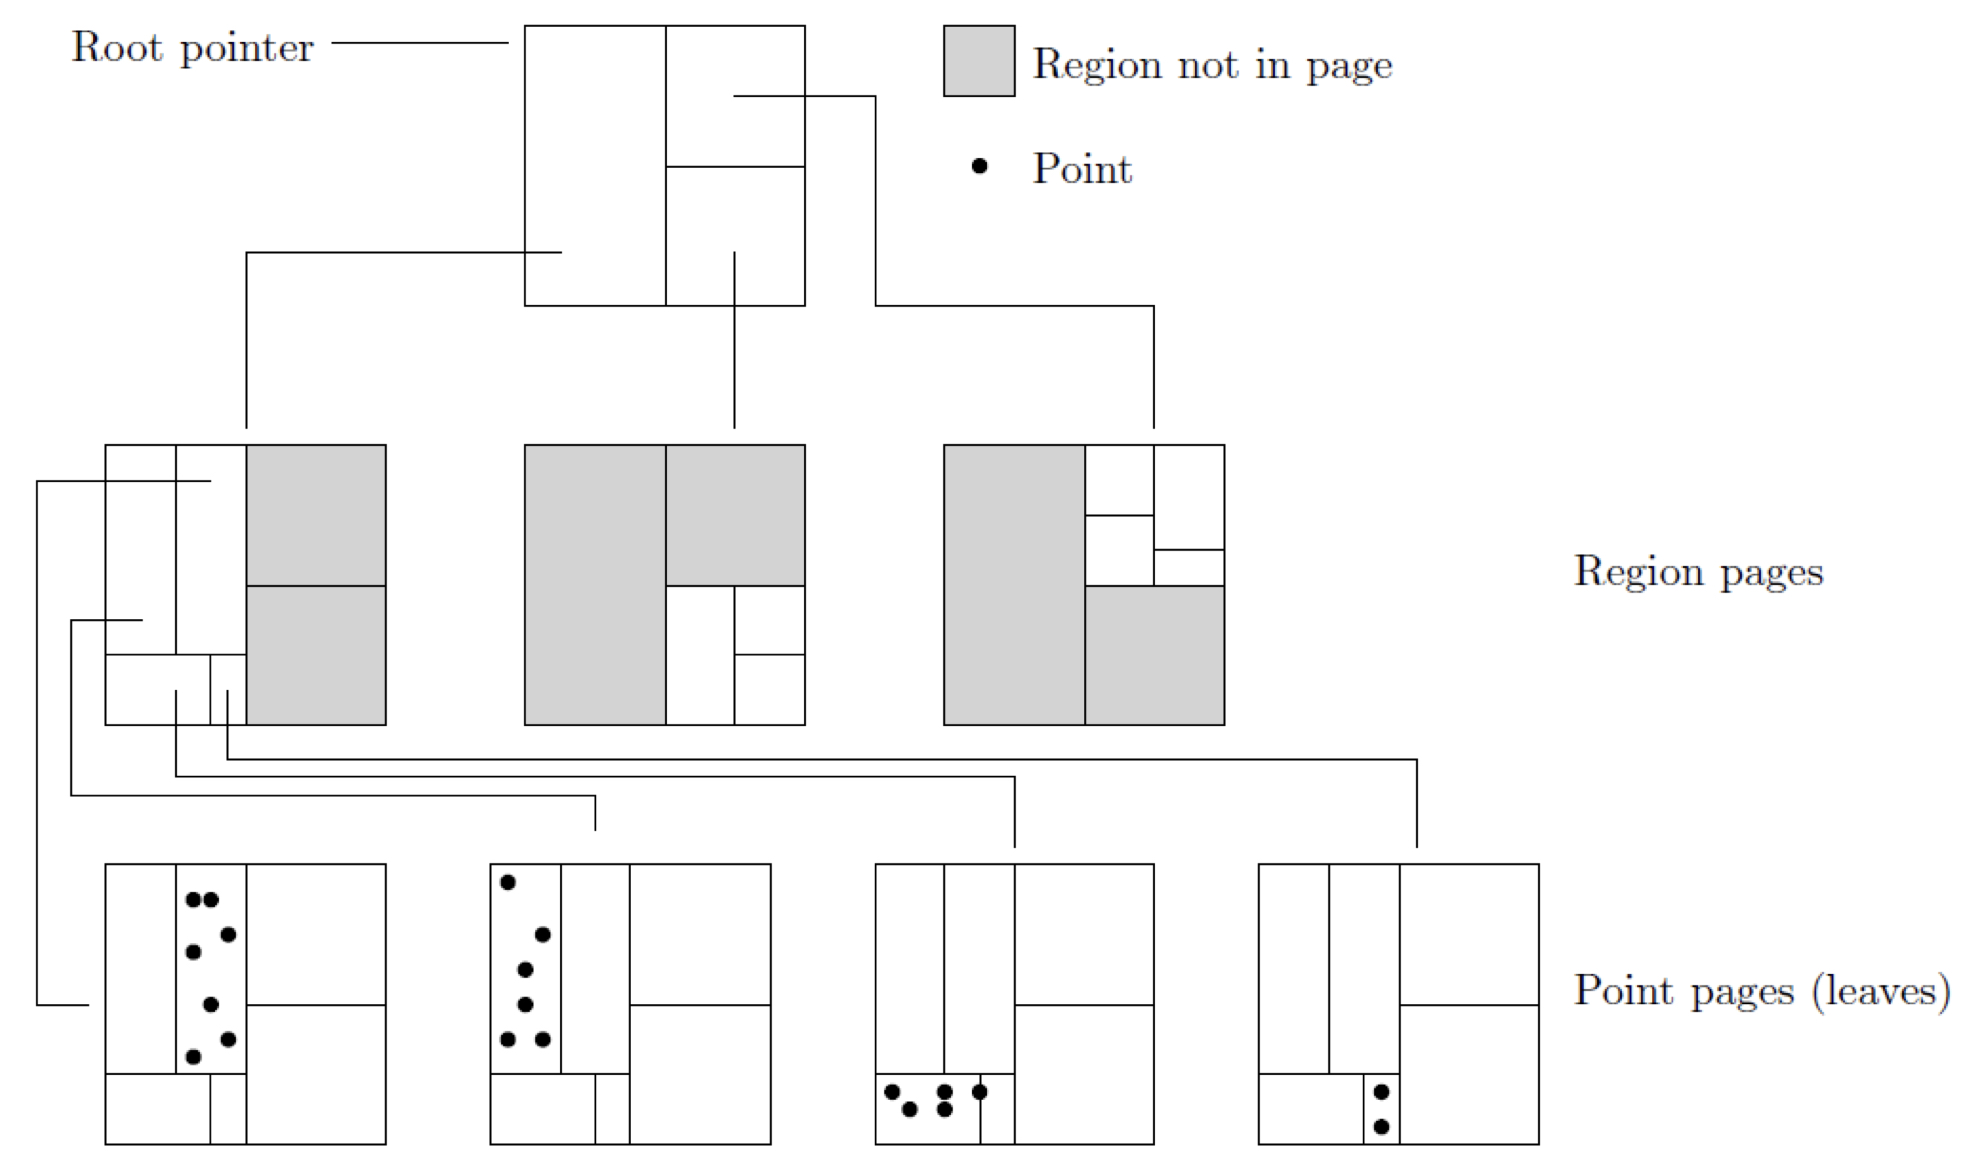
\includegraphics[width=.7\linewidth]{images/DBMS_Internals/MultiDimensionalDataOrganizations/kdb-tree.jpeg}
    \end{figure}
\end{itemize}

\section{G-trees}
The data space is divided into non-overlapping partitions of variable size identified by an appropriate \textbf{code}, then a total ordering is defined for partition codes, and they are stored in a B+–tree. A partition code is a binary string constructed as follows:
\begin{itemize}
    \item The initial region is identified by the empty string
    \item Splitting along side X, the two partition are identified by "0" and "1". 
    \begin{itemize}
        \item The points $0 < x \leq 50$ belong to partition "0"
        \item The points $50 < x \leq 100$ belong to partition "1"
    \end{itemize}
    \item In general a partition $R$ with the code $S$ is split, the sub-partition with values \textbf{less} than the half interval has the code $S“0”$ and that with values \textbf{greater} has the code $S“1”$.

    \newpage
    \begin{figure}[h]
         \centering
         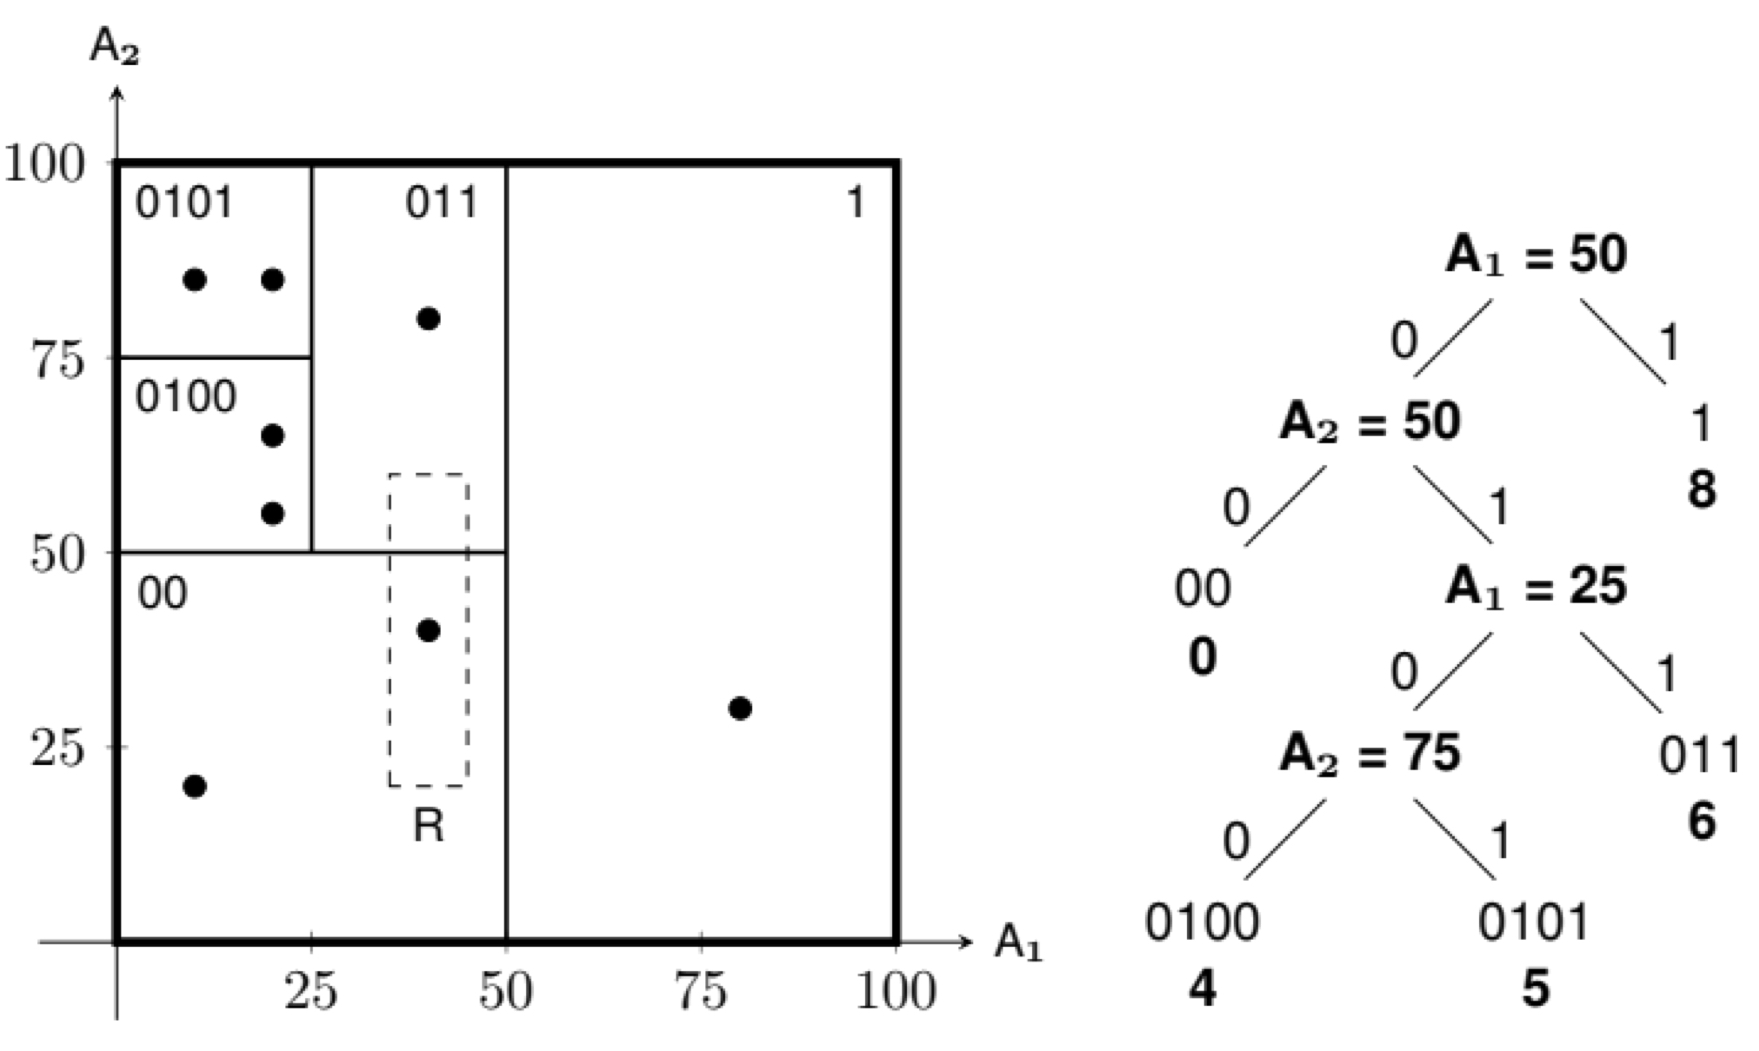
\includegraphics[width=.5\linewidth]{images/DBMS_Internals/MultiDimensionalDataOrganizations/G-tree1.jpeg}
    \end{figure}

    \begin{figure}[h]
         \centering
         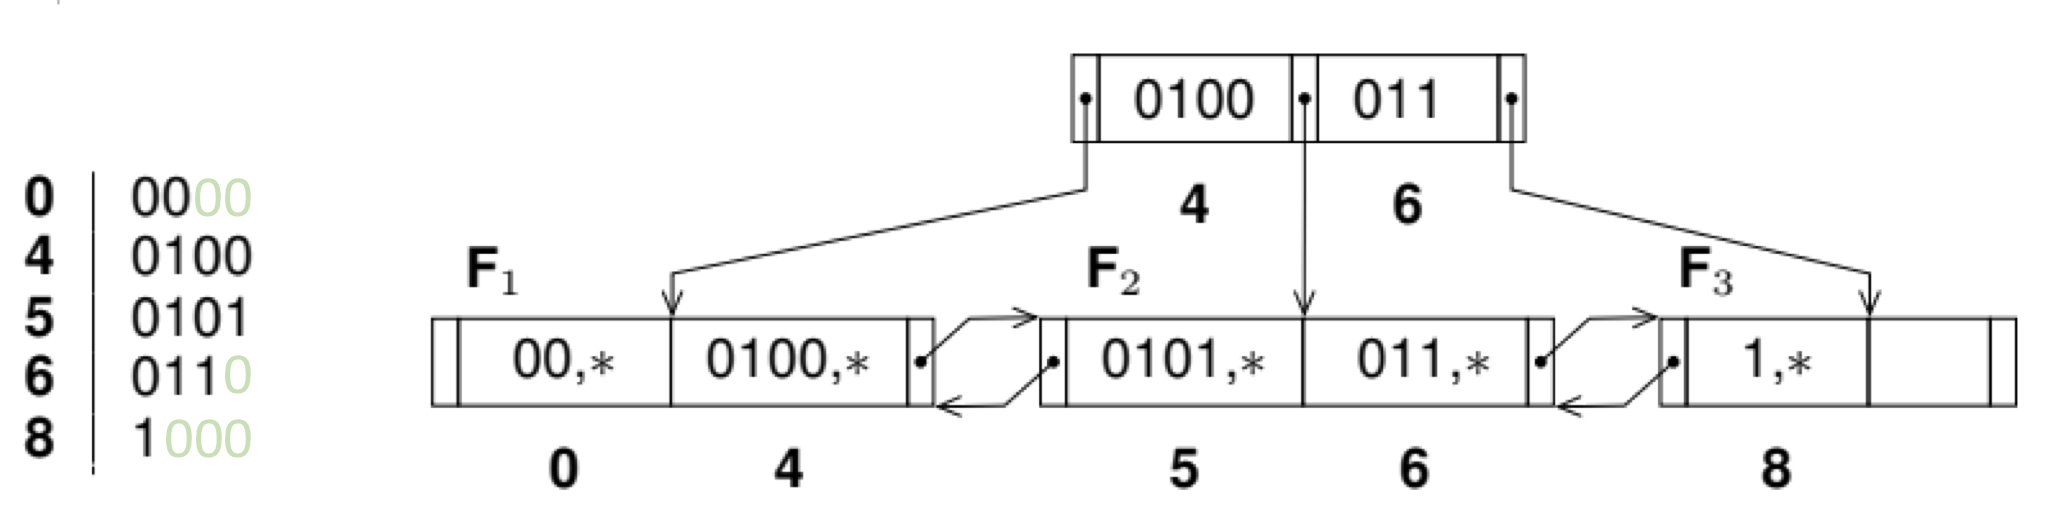
\includegraphics[width=.8\linewidth]{images/DBMS_Internals/MultiDimensionalDataOrganizations/G-tree2.jpeg}
    \end{figure}
    
\end{itemize}

Some important properties of the partition coding:
\begin{itemize}
    \item If a partition $R$ has the code $S$, the code of the partition from which $R$ has been created with one split is $S$ without the last bit
    \item The length of the code of a partition $R$ is the number of split made to get $R$ from the initial space
    \item Let \textit{RegionOf(S)} be a function that maps the code $S$ of a partition $R$ in the coordinates of the lower left and upper right vertices of the partition
\end{itemize}

\subsection{Point Search}
The search of a point $P$ with coordinates $(x, y)$ proceeds as follows:
\begin{enumerate}
    \item The partition tree is searched for the code $S_P$ of the partition that contains $P$, if it is present.
    \item The G–tree is searched for the partition code $S_P$ to check if $P$ is in the associated page
\end{enumerate}

\subsection{Spatial Range Search}
A spatial range search looks for the points $P_i$ with coordinates $(x_i, y_i)$ such that $x_1 \leq x_i \leq x_2$ and $y_1 \leq y_i \leq y_2$. The query result is found as follows:
\begin{enumerate}
    \item The G–tree is searched for the leaf node $F_h$ of the partition containing the \textbf{lower left} vertex $(x_1, y_1)$ of $R$
    \item The G–tree is searched for the leaf node $F_k$ of the partition containing the \textbf{upper right} vertex $(x_2, y_2)$ of $R$
    \item For each leaf from $F_h$ to $F_k$ the element's code $S$ are searched such that $R_S$ = \textit{RegionOf(S)} overlaps with the query region $R$
\end{enumerate}

\subsection{Point Insertion}
The insertion of a point $P$ with coordinates $(x, y)$ proceeds as follows:
\begin{enumerate}
    \item The G–tree is searched for the leaf node $F$ of the partition $R_P$ that should contain it. Let $S_P$ be the code of $R_P$
    \item If $R_P$ is not full, insert $P$, otherwise $R_P$ is split in $R_{P_1}$ and $R_{P_2}$, with codes $S_{P_1} = S_P$“0” and $S_{P_2} = S_P$“1”. If the new strings have a length greater than $M$, $M$ takes the value $M + 1$
    \item The points in $R_P$ and $P$ are distributed in $R_{P_1}$ and $R_{P_2}$
    \item The element $(S_P, p_{R_P})$ in the leaf $F$ is replaced by $(S_{P_1}, p_{R_{P_1}})$ and $(S_{P_2}, p_{R_{P_2}})$
\end{enumerate}

\subsection{Point Deletion}
The deletion of a point $P$ proceeds as follows:
\begin{enumerate}
    \item Let $F$ be the leaf node with the partition $R_P$ containing $P$, $S_P$ the partition code of $S_P$, and $S'$ the partition code of $R'$ obtained from $R_P$ with a split and therefore different from $S_P$ for the last bit only
    \item $P$ is deleted from $R_P$ and then two cases are considered:
    \begin{enumerate}
        \item \textit{$R'$ has been split:} 
        \begin{itemize}
            \item If the partition $R_P$ becomes empty, then $S_P$ is deleted
            \item Otherwise the operation terminates
        \end{itemize}
        \item \textit{$R'$ has not been split:}
        \begin{itemize}
            \item If the two partition cannot be merged, the operation terminates
            \item Otherwise the two partition are merged
        \end{itemize}
    \end{enumerate}
\end{enumerate}


\newpage
\section{R$^*$-trees}
\begin{figure}[h]
\centering
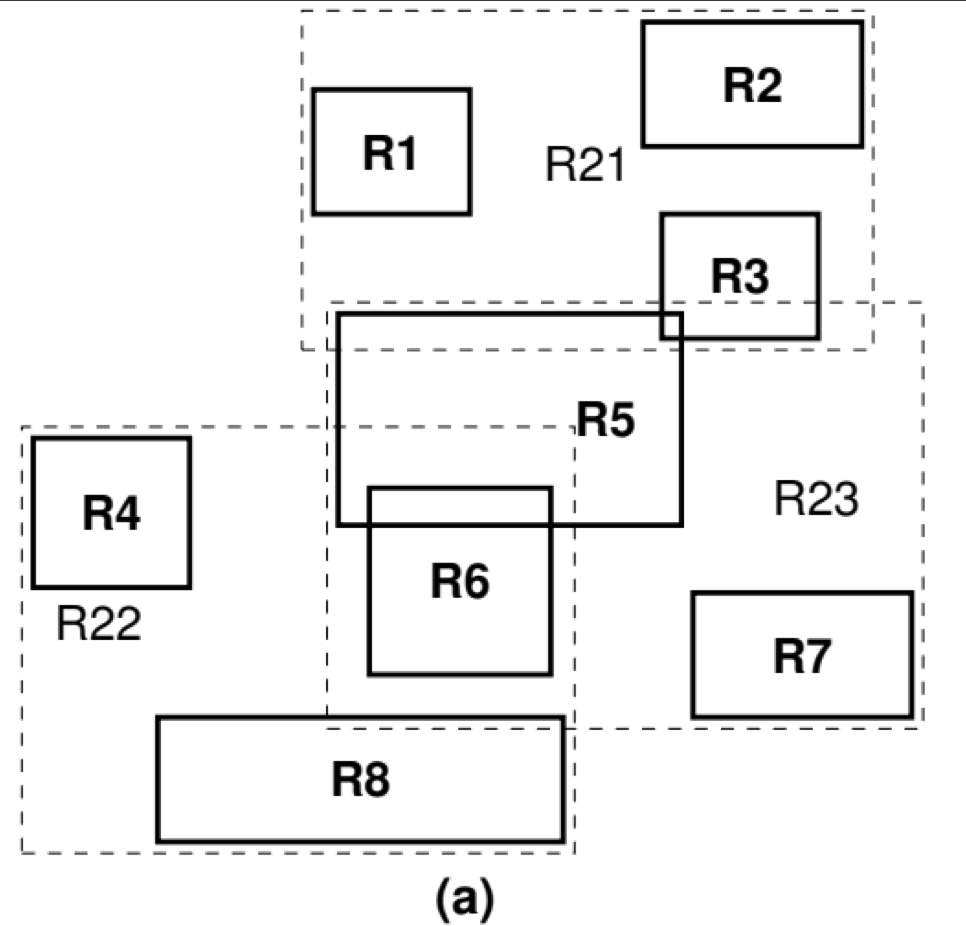
\includegraphics[width=.4\linewidth]{images/DBMS_Internals/MultiDimensionalDataOrganizations/r+tree1.jpeg}
\end{figure}
\begin{figure}[h]
\centering
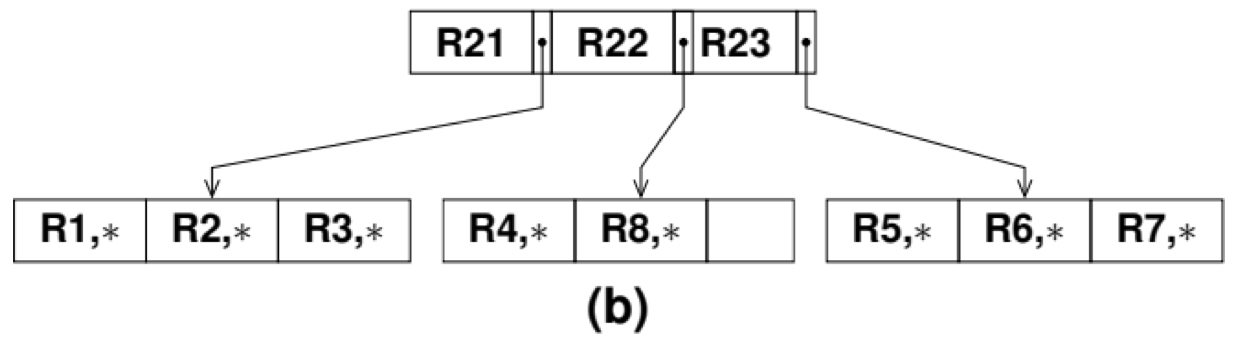
\includegraphics[width=.8\linewidth]{images/DBMS_Internals/MultiDimensionalDataOrganizations/r+tree.jpeg}
\end{figure}
\begin{itemize}
    \item Variant of R-tree, is a s a dynamic tree structure perfectly balanced as a B+–tree
    \item Rectangles described by the coordinates of the bottom left and the top right vertices
    \item Terminal nodes of a R*–tree contain elements of the form $(R_i, O_i)$
    \begin{itemize}
        \item $R_i$ is the rectangular data
        \item $O_i$ is a reference to the data nodes
    \end{itemize}
    \item The non-terminal nodes contain elements of type $(R_i, p_i)$
    \begin{itemize}
        \item $p_i$ is a reference to the root of a subtree
        \item $R_i$ is the minimum bounding rectangle containing all rectangles associated with the child nodes
    \end{itemize}
\end{itemize}



\subsection{Search Overlapping Data Regions}
The search of the data regions overlapping with $R$ proceeds as follows:
\begin{itemize}
    \item The root is visited in order to look for the elements $(R_i, p_i)$ with $R_i$ that overlaps with $R$
    \item For each element $(R_i, p_i)$ found, the search proceeds in a similar way in the subtrees rooted at $p_i$
    \item When a leaf node is reached, the data regions $R_i$ in the search result are those with $R_i$ that overlaps with $R$
\end{itemize}
\begin{figure}[h]
\centering
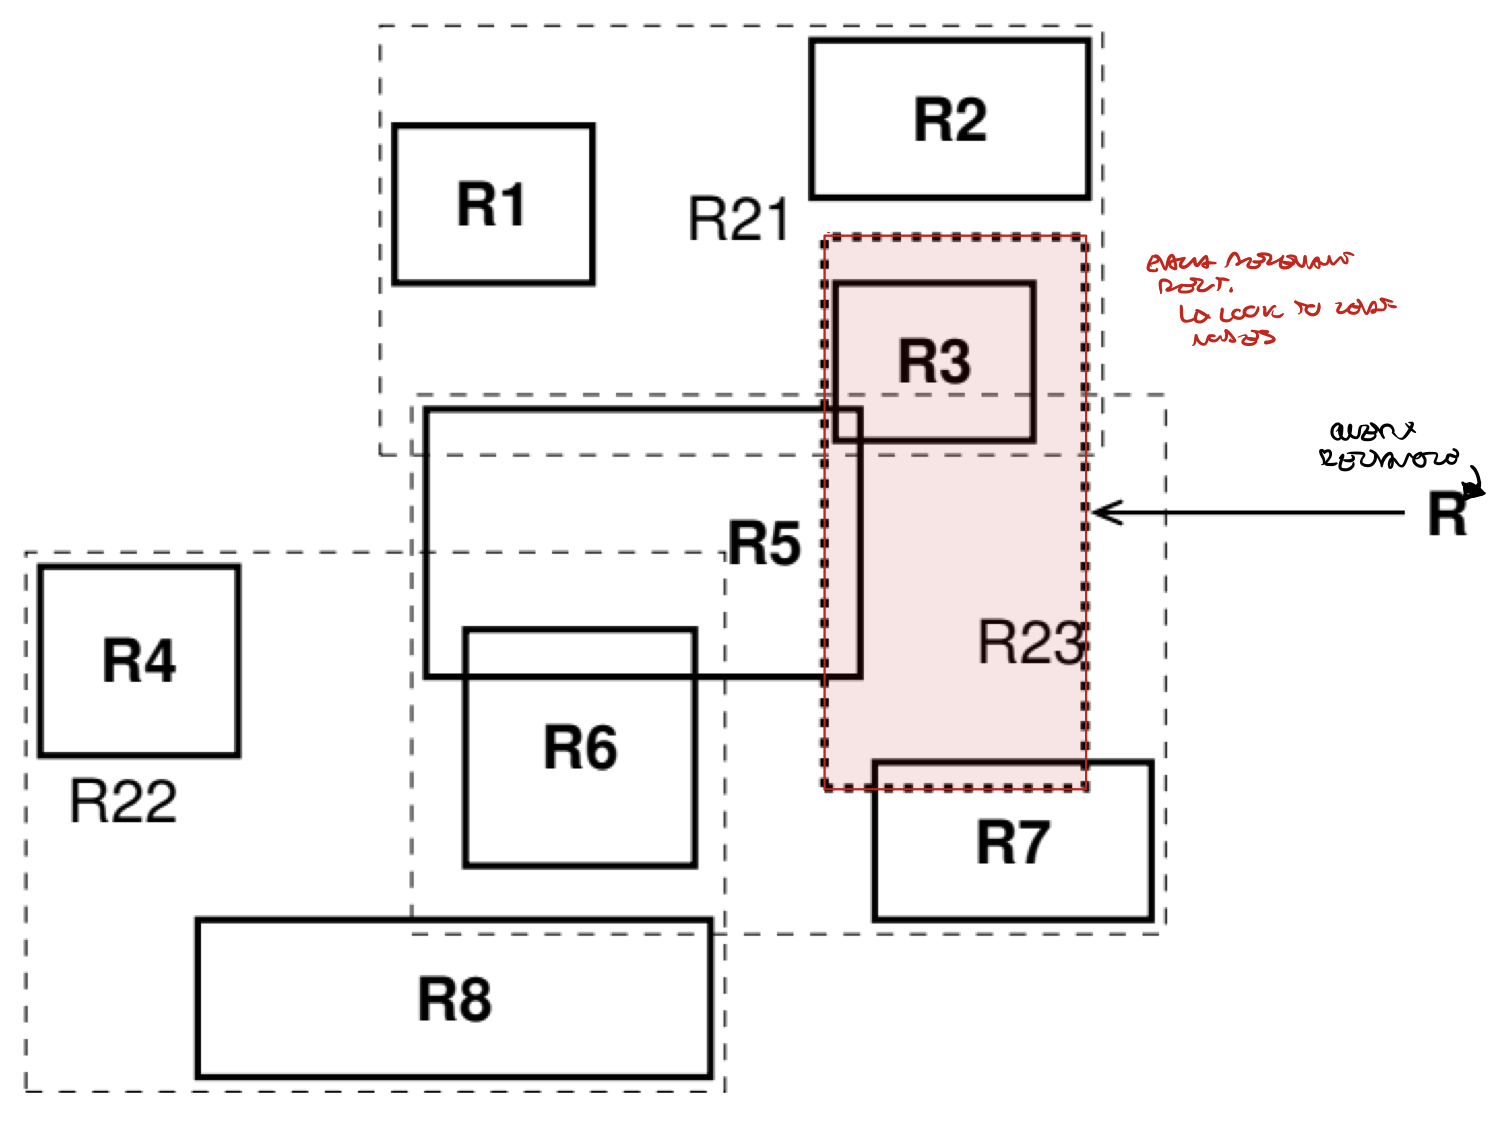
\includegraphics[width=.5\linewidth]{images/DBMS_Internals/MultiDimensionalDataOrganizations/r+tree2.jpeg}
\end{figure}

\subsection{Insertion}
Let $S$ be a new data region to insert in the tree. The operation is similar to inserting a key in a B+–tree since $S$ is stored into a leaf node, and if there is an overflow, the node will be split into two nodes. In the worst case the division can propagate to the parent node up to the root. The choice of the region in an internal node can be made according to the degree of overlap with S. After having selected the leaf node N where to insert S, if an overflow does not occur, the region is recalculated and its value propagates in the parent node. Otherwise, two cases are considered:
\begin{itemize}
    \item \textbf{Forced Reinsert:} If this is the first overflow from a leaf node, it is not split  instead $p$ of the $(M + 1)$ entries are removed from the node and reinserted in the tree
    \item \textbf{Node Splitting:} After the first overflow, the (M + 1) elements are divided between two nodes, and two new elements are inserted in the parent node, and the process goes on to propagate the effects
\end{itemize}
\begin{figure}[h]
\centering
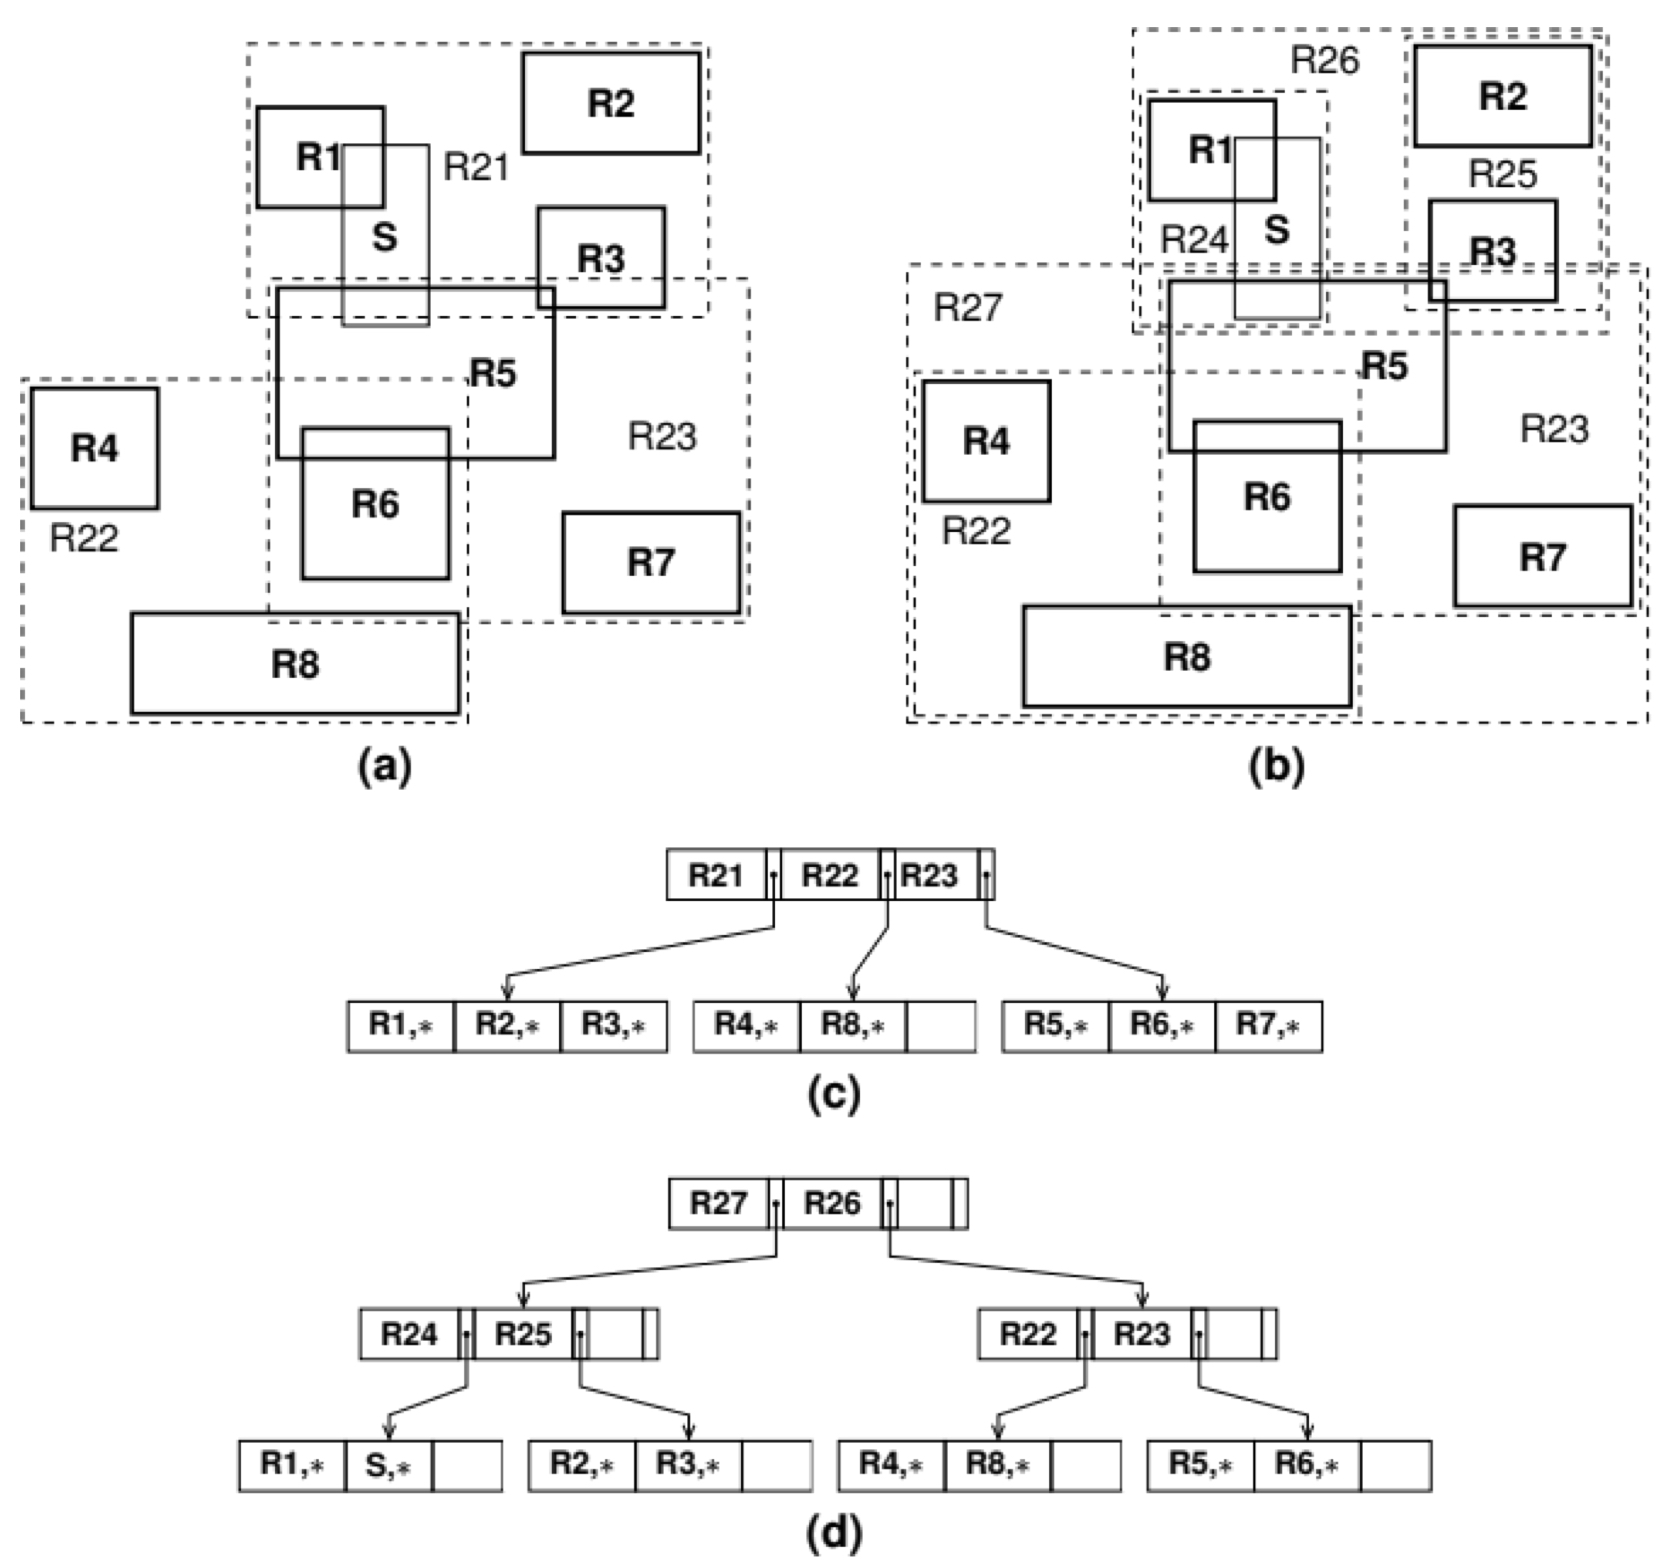
\includegraphics[width=.5\linewidth]{images/DBMS_Internals/MultiDimensionalDataOrganizations/r+tree3.jpeg}
\end{figure}